% Typeset with XeLaTeX
% Allows use of system fonts rather than just LaTeX's ones
% NOTE - if you use TeXShop and Bibdesk (Mac), can complete citations
%  - open your .bib file, type \citep{xx... and then F5 or Option-Escape
\documentclass[12pt]{article} % 12pt with Minion Pro
% for NIH - print this PDF at 104% to be sure it's no more than 15 characters
%  per inch and no less than 6 lines per inch (with Minion Pro 12pt)
\usepackage{geometry} % set page layout
% this gives reasonable margins for NIH forms after the 104% print
\geometry{left=0.8in,right=0.8in, top=0.8in, bottom=0.8in,letterpaper}  
\usepackage[xetex]{graphicx} % allows us to manipulate graphics.
% Replace option [] with pdftex if you don't use Xe(La)TeX
\usepackage{color}
%\usepackage{hyperref}
\usepackage{epstopdf} % automatic conversion of eps to pdf 
\usepackage{amsmath, amssymb} % Better maths support & more symbols
\usepackage{enumitem}[shortlabels] % control over indentation for enumerate etc.
\usepackage{textcomp} % provide lots of new symbols - see textcomp.pdf
%\usepackage{enumerate}% http://ctan.org/pkg/enumerate
% line spacing: \doublespacing, \onehalfspacing, \singlespacing
\usepackage{setspace}
\singlespacing
\setstretch{0.95} % shrink line spacing a little bit
% allows text flowing around figs
% use \begin{wrapfigure}{x}{width} where x = r(ight) or l(eft)
\usepackage{wrapfig}
\usepackage{floatflt}
\usepackage{relsize}
\usepackage[parfill]{parskip} % don't indent new paragraphs
%\usepackage{flafter}  % Don't place figs & tables before their definition 
\usepackage{verbatim} % allows \begin and \end{comment} regions
\usepackage{booktabs} % makes tables look good
\usepackage{bm}  % Define \bm{} to use bold math fonts
% linenumbers in L margin, start & end with \linenumbers \nolinenumbers,
\usepackage{lineno} % use option [modulo] for steps of 5
\usepackage[auth-sc]{authblk} % authors & institutions - see authblk.pdf
\renewcommand\Authands{ and } % separates the last 2 authors in the list
% control how captions look; here, use small font and indent both margins by 20pt
% margin option doesn't seem to work with wrapfig
\usepackage[margin=0pt,size=footnotesize, labelfont=bf, labelsep=colon]{caption}

\usepackage{sidecap}
%\usepackage[capbesideposition=outside,capbesidesep=quad]{floatrow}

 % Nice tables
\usepackage{colortbl}% http://ctan.org/pkg/colortbl
\usepackage{xcolor}% http://ctan.org/pkg/xcolor
\colorlet{tablerowcolor}{gray!10} % Table row separator colour = 10% gray
\newcommand{\rowcol}{\rowcolor{tablerowcolor}}
 
 
%:FONT
% If you don't want to use system fonts, replace from here to 'Citation style' with \usepackage{Palatino} or similar
\usepackage[no-math]{fontspec} % 'no-math' = keep computer modern for math fonts unless you say differently below
\usepackage{xunicode} % needed by XeTeX for handling all the system fonts nicely
\usepackage[no-sscript]{xltxtra} 
%\setmonofont[Scale=0.8]{Lucida Sans} % typeface for \tt commands
%\setsansfont[BoldFont={Lucida Sans Demibold Roman}, ItalicFont={Lucida Sans Italic}]{Lucida Sans} %my choice of sans-serif font
\defaultfontfeatures{Mapping=tex-text} % convert LaTeX specials (``quotes'' --- dashes etc.) to unicode, to preserve them
%\setmainfont[BoldFont={Minion Pro Bold.otf}, ItalicFont={Minion Pro Italic.otf}]{Minion Pro Reg.otf} %%% for overleaf
\setmainfont{Minion Pro}
%\setmainfont{Arial}

%:CITATION STYLE
% natbib package: square,curly, angle(brackets)
% colon (default), comma (to separate multiple citations)
% authoryear (default),numbers (citations style)
% super (for superscripted numerical citations, as in Nature)
% sort (orders multiple cites into order of appearance in ref list, or year of pub if authoryear)
% sort&compress: as sort, + multiple citations compressed (as 3-6, 15)
\usepackage[numbers,super,sort&compress]{natbib}

%:NUMBERING STYLE FOR BIBLIOGRAPHY
% (e.g, here it will be 1. and not [1] as in standard LaTeX)
\makeatletter
\renewcommand\@biblabel[1]{#1.}
\makeatother

%:SHORTCUT COMMANDS
% Maths
\newcommand{\ddt}[1]{\ensuremath{\frac{{\rm d}#1}{{\rm d}t}}}  % d/dt
\newcommand{\dd}[2]{\ensuremath{\frac{{\rm d}#1}{{\rm d}#2}}} % dy by dx  - \dd{y}{x}
\newcommand{\ddsq}[2]{\ensuremath{\frac{{\rm d}^2#1}{{\rm d}#2^2}}} % second deriv
\newcommand{\pp}[2]{\ensuremath{\frac{\partial #1}{\partial #2}}} % partial \pp{y}{x}
\newcommand{\ppsq}[2]{\ensuremath{\frac{\partial^2 #1}{\partial {#2}^2}}}
\newcommand{\scinot}[2]{\ensuremath{#1 \times 10^{#2}$}}
\newcommand{\superscript}[1]{\ensuremath{^{\textrm{#1}}}} %normal (non-math) font for super/subscripts in text
\newcommand{\subscript}[1]{\ensuremath{_{\textrm{#1}}}}
\newcommand{\posi}{\ensuremath{^+}}
\newcommand{\nega}{\ensuremath{^-}}
% Text
\newcommand{\khi}{\ensuremath{\text{Ki67}^\text{hi}}}
\newcommand{\klo}{\ensuremath{\text{Ki67}^\text{lo}}}
\newcommand{\poseight}{\ensuremath{\text{CD8}^+}}
\newcommand{\posfour}{\ensuremath{\text{CD4}^+}}
\newcommand{\trm}{T$_\text{RM}$}
\newcommand{\tcm}{T$_\text{CM}$}
\newcommand{\tem}{T$_\text{EM}$}
\newcommand{\treg}{T$_\text{reg}$}
\newcommand{\tvm}{T$_\text{VM}$}

\newcommand{\tighten}{\vspace{-0.35cm}}
\newcommand{\tightenabit}{\vspace{-0.15cm}}

\newcommand{\khishort}{Ki67$^\text{high}$}
\newcommand{\kloshort}{Ki67$^\text{low}$}
\newcommand{\bpos}{BrdU$^\text{pos}$~}
\newcommand{\bneg}{BrdU$^\text{neg}$~}
\newcommand{\bposshort}{BrdU$^\text{pos}$}
\newcommand{\bnegshort}{BrdU$^\text{neg}$}


% how to highlight my name in reference lists - choose one of the following
\newcommand{\myemphasis}[1]{\textbf{\underline{#1}}} 
%\newcommand{\myemphasis}[1]{\textsc{#1}} % small caps
%\newcommand{\myemphasis}[1]{\textbf{#1}} % bold

\newcommand{\myname}{\myemphasis{Andrew J. Yates}}

% how you want volume of journals to look
\newcommand{\volume}[1]{\textbf{#1}} 
\newcommand{\bi}{\begin{itemize}}
\newcommand{\ei}{\end{itemize}}

% Formatting
\newcommand{\para}[1]{\vspace*{-4.5mm}\paragraph{#1}}
% Editing
\newcommand{\red}[1]{{\color{red}{#1}}}
\newcommand{\blue}[1]{{\color{blue}{#1}}}
\newcommand{\cyan}[1]{{\color{cyan}{#1}}}
% Standard stuff
\newcommand{\be}{\begin{equation}}
\newcommand{\ee}{\end{equation}}
\newcommand{\bea}{\begin{eqnarray}}
\newcommand{\eea}{\end{eqnarray}}

\renewcommand\refname{Cited literature}
%% \begin{graybox} text \end{graybox} for text with a background colour
%\definecolor{MyGray}{rgb}{0.96,0.97,0.98}
%\definecolor{MyGray}{rgb}{0.96,0.90,0.98}
%\makeatletter\newenvironment{graybox}{%
%   \begin{lrbox}
%   {\@tempboxa}\begin{minipage}[r]{0.98\columnwidth}}{\end{minipage}\end{lrbox}%
%   \colorbox{MyGray}{\usebox{\@tempboxa}}
%}\makeatother

%%%%%%%%%%%%%%%%%%%%%%%%%%


\usepackage{url}\newcommand\hi{$^\text{high}$}
\newcommand\lo{$^\text{low}$}



% diagrams in latex
\usepackage{tikz}
\usetikzlibrary{shapes.geometric, arrows}
\tikzstyle{box1} = [rectangle, rounded corners, minimum width=2cm, minimum height=1cm, text centered, draw=black, fill=green!60]
\tikzstyle{box2} = [rectangle, rounded corners, minimum width=2cm, minimum height=1cm, text centered, draw=black, fill=green!30]
\tikzstyle{box3} = [rectangle, rounded corners, minimum width=2cm, minimum height=1cm, text centered, draw=black, fill=yellow!60]
\tikzstyle{box4} = [rectangle, rounded corners, minimum width=2cm, minimum height=1cm, text centered, draw=black, fill=blue!30]
\tikzstyle{box5} = [rectangle, rounded corners, minimum width=2cm, minimum height=1cm, text centered, draw=black, fill=blue!60]


%%%%%%%%%%%%%%%%%%%%%%%%%%

\begin{document}
%\relscale{1.08} % or whatever scaling is desired
\pagestyle{empty}

\setlength{\parskip}{1.5mm}


\subsection*{Modelling the dynamics of timestamped naive CD8 T cells in neonates and adults.}
\vspace{0.2cm}

To further discriminate the adaptation and quorum-sensing mechanisms, we compared their ability to explain data from diverse experimental settings. 
In that attempt we turn to a previously published dataset by Reynaldi et. al., who have developed a beautiful system to study the effects of host and cell age on naive CD8 T cell dynamics.
They used a tamoxifen driven CD4-Cre$^{ERT2}$ RFP reporter mouse model to track the cohorts of CD8 T cells exported from the thymus in animals of varying ages.
%When these mice are treated with tamoxifen, expression of RFP is induced in all CD4 expressing cells.
This strategy was used to label CD8 T cells in their double positive (CD4$^{+}$ CD8$^{+}$) thymic developmental stage, when they briefly express CD4.
Tamoxifen treatment was then used to mark CD8 T cells with a timestamp of their thymic export.
Treating animals of different ages with tamoxifen and following RFP labelled cohorts as they age in the periphery allows to draw inferences on effects of host and/or cell age on CD8 T cell dynamics under homeostatic conditions (Figure~\ref{fig:timestamp_strategy}).

\begin{figure}[htbp]
\centering
  %\vspace*{-2mm}
      %\includegraphics[width=\textwidth]{ts_strategy1.png}
      \includegraphics[scale=0.5]{ts_strategy1.png}
      \caption{\textbf{Fate mapping naive CD8 T cells.}}
   \label{fig:timestamp_strategy}
 \end{figure}

In each animal, the initial pool size of labelled cells ($N_{0}$) was measured 2 weeks after the tamoxifen treatment and its homeostatic loss was followed in blood by serial sampling.
The time course of RFP labelled cells revealed that the loss of CD8 T cells slows down with their age (Figure~\ref{fig:timestamp_data}, the slopes of cell counts within each group). % change cohort to group in the figure.
Additionally there is a hint of quicker loss of recently emigrated cells in neonates as compared to in adult mice (Figure~\ref{fig:timestamp_data}, cell loss from 1st time-point to the second within each cohort).

\begin{wrapfigure}{r}{0.60\textwidth}
\centering
\vspace*{-4mm}
     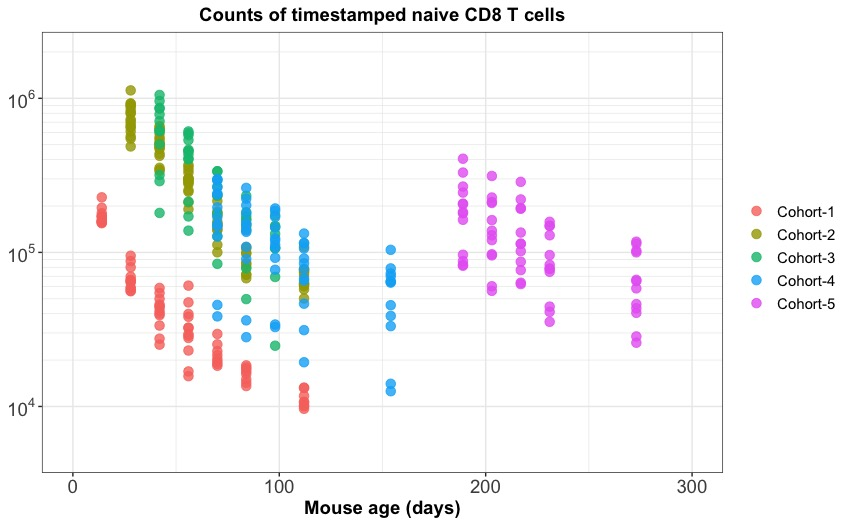
\includegraphics[width=0.60\textwidth]{tmstmp_data.jpeg}
      \caption{\textbf{Total Counts of timestamped naive CD8 T cells in CD4-Cre$^{ERT2}$ reporter mice treated with tamoxifen at different host ages.}}
   \label{fig:timestamp_data}
  \vspace*{-4mm}
 \end{wrapfigure}

In the data structure, where cellular dynamics are compared on repeat samples drawn from animals in distinct treatment groups (different color cohorts in Figure~\ref{fig:timestamp_data}), random effects due to non-independence are needed to be accounted using multi-level mathematical models.
We do this by pooling information within and among groups by assuming animal and/or group level variation in the initial count of RFP labelled cells ($N_{0}$) and in the loss rate of youngest cells in the periphery ($\lambda_{0}$ for cells of age 0) in a hierarchical modeling approach. 
We then compare the ability of age-structured and density-dependent models to explain this multi-level data using the Bayesian statistical methods.

\subsection*{Hierarchical age-structured model}
We model the loss of RFP labelled naive CD8 T cells by assuming that their net loss rate varies with their time since thymic export (cell age) such that $\lambda(a) = \lambda_{0} e^{-\gamma\,a}$.
The dynamics of cells of age `a' at different host ages `t' then can be followed using a PDE,
\begin{equation}
\begin{aligned}
\frac{\partial N}{\partial t} + \frac{\partial N}{\partial a} = -\lambda(a) \,\, N(t, a), 
\end{aligned}
\label{eq:pde-asm}
\end{equation}
Here, the net loss rate $\lambda$ is an aggregate effect division of CD8 T cells and their loss by death and differentiation into memory T cells.


To fit the age-structured model (equation~\ref{eq:pde-asm}) to the multi-level data from Reynaldi et. al., we defined different permutations of either $N_{0}$ and $\lambda_{0}$ as normally distributed hyper-parameters varying across the treatment groups and/or animals in a nested modelling scheme.
The mean and sigma of these distributions are then estimated from the data along with the free parameter $\gamma$.%, which is the rate of change of $\lambda$ with cell age.
The general strategy of hierarchical modeling is defined in (equation~\ref{eq:hierrarch}), where we formulate the likelihood of data ($y$) by assuming that the errors in our model predictions ($\mu$) are normally distributed.

\begin{eqnarray}
\begin{aligned}
&y_i \sim \text{normal}(\mu_i, \sigma) \quad \quad \quad \quad \quad \quad  &[\text{likelihood}] \\
&\mu_i = f(t_i, N_0, \lambda_0, \gamma)  &[\text{model}]\\
\\
&\textbf{Hyper parameters} \\
&N_0 \sim \text{normal}(\mu_N, \sigma_N) \quad \quad \quad  &[\text{Initial counts}]  \\
&\lambda_0 \sim \text{normal}(\mu_{\lambda}, \sigma_{\lambda})   &[\text{Loss rate at cell-age=0}]\\
%\\
%&\gamma \sim \text{normal}(0.05, 0.01) &[\gamma \text{ prior}]
\end{aligned}
\label{eq:hierrarch}
\end{eqnarray}

We define priors for $\mu_{N}, \sigma_{N}, \mu_{\lambda}, \sigma_{\lambda}$ and $\gamma$ and fit individual permutations of the hierarchical age-structured model to the time-course of labelled CD8 T cell counts separately.
The $\Delta$Loo-IC values of the hierarchical age-structured models are shown in table~\ref{tab:stats-hierrarch}.
The model in which the initial count of labelled cells is varied among mice and the loss rate of youngest cells is varied among different tamoxifen-treatment groups emerges as the best-fitting model with 100\% relative statistical support from the data.
This suggests that there is a substantial variation in tamoxifen-driven labelling among treated mice (Figure~\ref{fig:timestamp_N0}), which is expected given the dynamic variation in thymic cellularity (proxy for the thymic export) across the mouse lifespan. 
Strikingly, the group-level variation in $\lambda_0$ (Figure~\ref{fig:timestamp_L0}A), shows a substantial decline in the loss rate of RTEs as a function of host age (Figure~\ref{fig:timestamp_L0}B).
%follows a distinct pattern of higher loss rate in neonates as compared to in adult mice, .

%: Table 2
	\begin{table}[h!]
		\begin{center}
			\renewcommand{\arraystretch}{1.25}
			\begin{tabular}{ l c c } 
				\toprule 
				\textbf{Model}  &  {$\Delta$Loo-IC}  &  {Akaike weight\%} \\ 
				\toprule
				$N_{0}$ varying at animal level                                               & 316    &  0.0   \\
				$N_{0}$ varying at animal level; $\lambda_{0}$ varying at group level         & \cyan{\textbf{0.0}}    &  \cyan{\textbf{100}}  \\
				$N_{0}$ varying at animal level; $\lambda_{0}$ varying at animal level        & 73     &  0.0  \\
				$N_{0}$ varying at group level; $\lambda_{0}$ varying at animal level         & 313    &  0.0  \\ 
				\hline
				\toprule 
			\end{tabular}
		\end{center}
		\caption{\small \textbf{Statistical support for the hierarchical age-structured models.}
		\label{tab:stats-hierrarch}}
	\end{table} 

\clearpage

\begin{wrapfigure}[13]{l}{0.54\textwidth} 
\centering
     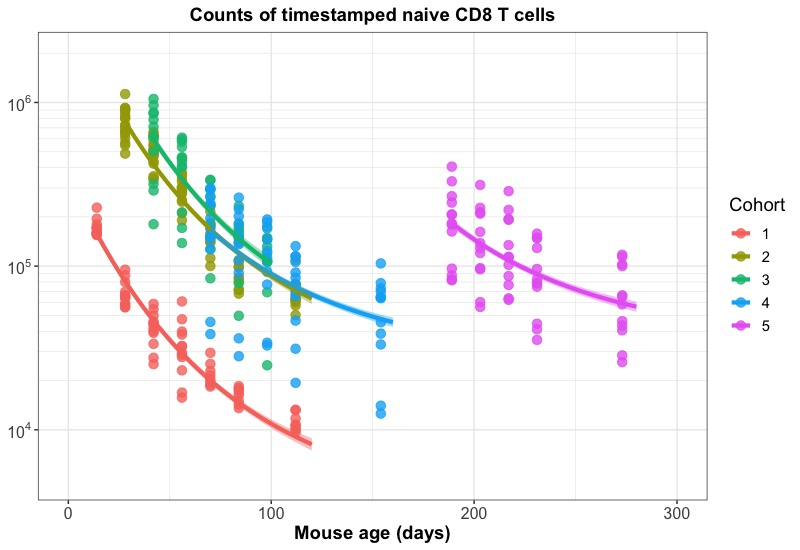
\includegraphics[width=0.53\textwidth]{model_fit_lambdaHA_sigmoid.jpeg}
      \caption{\textbf{Model fit using equation~\ref{eq:lambda-host-cell-age} to labelled CD8 counts.}}
   \label{fig:timestamp_fit}
   \end{wrapfigure}
 
We captured the host age dependent variation in $\lambda_0$ by defining a phenomenological function and used it to derive the general form of net loss rate of cells of age `a' at time `t',

\begin{equation}
\begin{aligned}
\lambda(t, a) = \, &\lambda_h \, \bigg(1 + \frac{Q}{1 + (t/q1)^5} \bigg) \, e^{-\gamma \, a}.\\
&----  \lambda_0 ----
\end{aligned}
\label{eq:lambda-host-cell-age}
\end{equation}

We replaced the group-level variation in $\lambda_0$ using the equation~\ref{eq:lambda-host-cell-age} and found that this modified model explained the data equally well ($\Delta$ LOO-IC $\sim 6$ and Figure~\ref{fig:timestamp_fit}).
We estimated the parameters $\lambda_h, Q, q1$ and $\gamma$ to derive the precise form net loss rate of CD8 T cells of age `a' across the mouse life-span.
 
\begin{figure}[htbp]
\centering
  %\vspace*{-2mm}
      \includegraphics[scale=0.45]{tmstmp_L0.png}
      \caption{\textbf{Variation in the net loss rate of CD8 RTE among treatment groups.}}
   \label{fig:timestamp_L0}
 \end{figure}

	

\begin{figure}[htbp]
\centering
  %\vspace*{-2mm}
      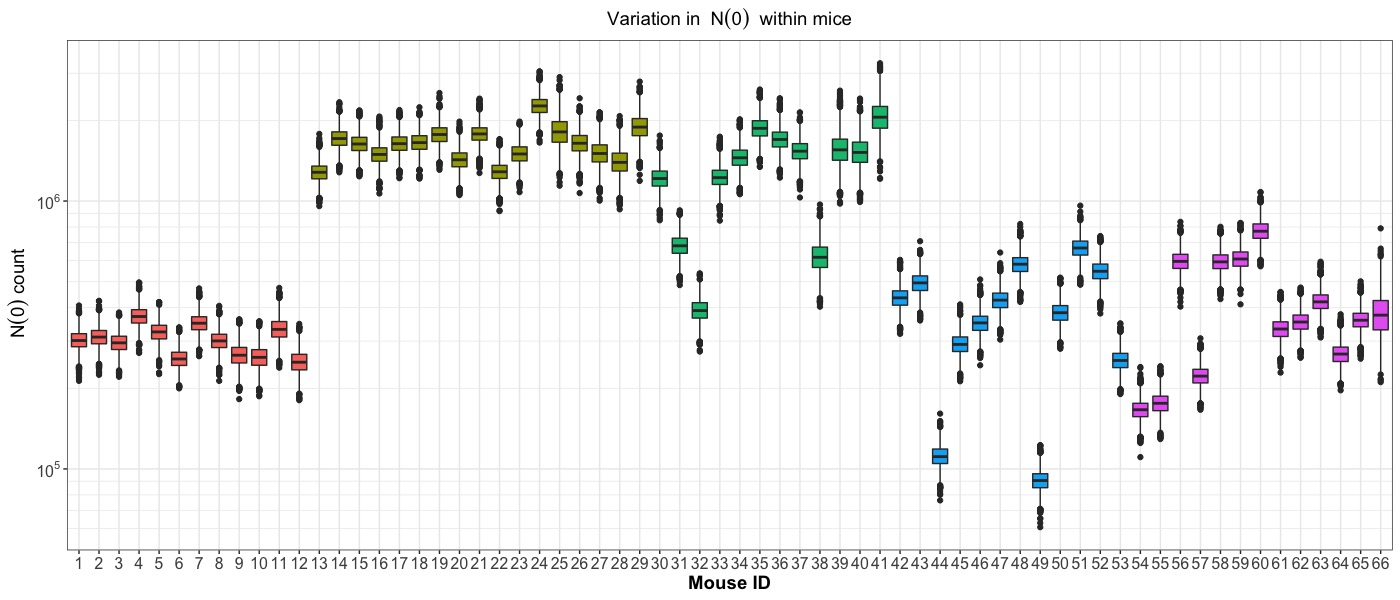
\includegraphics[width=\textwidth]{tmstmp_N0.jpeg}
      \caption{\textbf{Variation in initial labelling of CD8 T cells among mice.}}
   \label{fig:timestamp_N0}
 \end{figure}


\end{document}
